\subsection{Unnecessary Abstraction}
    \textit{Unnecessary Abstraction} (\textit{UNA}), definito da G. Suryanarayana et al. \cite{SURYANARAYANA201521}, si verifica quando un \textit{abstraction} che non è in realtà necessaria (e quindi potrebbe essere evitata) viene introdotta nel design.
    Questo \textit{smell} viola il principio di astrazione, poiché si verifica l'introduzione nel design di \textit{abstraction} con responsabilità limitate oppure nulle.
    
    Si possono riassumere tre cause principali che portano l'introduzione di questo \textit{smell} nel design:
        %Le cause principali dell'introduzione di questo \textit{smell} nel sistema si possono riassumere in tre differenti casi:
    \begin{itemize}
        \item \textit{Utilizzo improprio di feature del linguaggio:}
        \textit{abstraction} non necessarie possono essere introdotte nel design solamente per convenienza, utilizzando \textit{feature} del linguaggio in maniera impropria. Il caso più diffuso è rappresentato dalle \textit{constant placeholder}, interfacce o classi utilizzate dal programmatore solamente per contenere valori costanti.
        La generazione di queste \textit{abstraction} consente al programmatore di implementare o estendere il \textit{placeholder} nella classe desiderata in modo da utilizzare una costante senza la necessità di specificarne il tipo ma solamente attraverso il suo nome.
        
        \item \textit{Over-engineering:} vengono definite \textit{over engineered} le \textit{abstraction} introdotte nel design che risultano superflue e prive di un grande significato associato. 
        Un esempio di classe over engineered è mostrato dalla figura 3, dove sono presenti una classe \textit{Customer} contenente un attributo ID che, invece di essere di tipo \textit{String}, è incapsulato da una classe \textit{CustomerID} dedicata, superflua e non necessaria per il sistema.
        %Un esempio di questo caso può essere rappresentato da una classe Customer contenente un attributo CustomerID che, al posto di essere un attributo \textit{String} di Customer, ha una classe CustomerID dedicata che presenta getter e setter, costruttore e appunto un parametro ID di tipo \textit{String}. CustomerID risulta quindi superflua e non necessaria per il sistema.
        \begin{figure}[h]
            \centering
            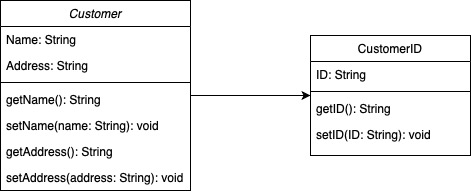
\includegraphics[scale=0.45]{Tesi/Sezione3-RiconoscimentoSmell/immagini/Untitled Diagram.jpg}
            \caption{Esempio di classe over engineered}
            \label{fig:my_label}
        \end{figure}
        
        
        \item \textit{Procedural thinking:} %si verifica quando lo sviluppatore, soprattutto se sè è affacciato di recente allo sviluppo object-oriented, tende a pensare le classi in modo procedurale.
        se uno sviluppatore, spesso affacciato recentemente allo sviluppo Object Oriented, tende a pensare le classi in maniera procedurale e non dotate di responsabilità e compiti, può introdurre nel codice \textit{abstraction} non necessarie. 
        Questa tendenza si traduce in classi che "svolgono procedure" invece di "essere qualcosa" violando il principio di astrazione, a causa di responsabilità multiple e poco definite. Un esempio di classe procedurale possono essere le classi di \textit{utilities}.
    \end{itemize}
    
    
    \paragraph{Nodo di tipo smell nel grafo}
        Il nodo dello \textit{smell} presenta un'unica dipendenza verso la sospetta \textit{Unnecessary Abstraction}. Inoltre ha una proprietà chiamata \textit{unnecessaryCase}, che indica quale delle tre casistiche di \textit{UNA} è stata riscontrata nella \textit{unit}.
        
            
    %Problemi e refactoring
    \subsubsection{Impatto sulla qualità del codice e refactoring}
        \textit{Unnecessary Abstraction} ha un impatto significativo sulla possibilità di riutilizzo del codice e sulla comprensione del progetto. 
        Riguardo la comprensione, la presenza di numerose interfacce non necessarie incide in maniera negativa poiché aumenta la complessità del design, causando una maggiore difficoltà nell'interpretazione del design e nella chiarezza del progetto.
        
        Anche il riutilizzo del codice subisce un influenza negativa dalla presenza di \textit{Unnecessary Abstraction} poiché \textit{abstraction} senza responsabilità uniche e ben definite e specializzate per un design particolare risultano molto difficili da riutilizzare in contesti differenti.
        
        Se inoltre viene utilizzata un'interfaccia come \textit{constant placeholder} possono verificarsi ulteriori problemi:
        \begin{itemize}
            \item Le classi derivate da quelle che implementano l'interfaccia possono risultare inquinate da costanti che non sono rilevanti per loro.
            
            \item Si verifica una violazione dell'incapsulamento in quanto vengono mostrati, attraverso l'interfaccia, dettagli implementativi.
            
            \item Quando le costanti sono presenti nelle interfacce, cambiamenti ad esse possono creare problemi ai \textit{client} esistenti.
            
            \item Le interfacce rappresentano un protocollo che le classi che lo implementano devono rispettare e l'utilizzo come \textit{constant placeholder} è un abuso del meccanismo di astrazione.
        \end{itemize}
        
        Al fine di rimuovere questo problema dal codice ed aumentare la qualità dello stesso, sono suggerite tre diverse strategie \cite{SURYANARAYANA201521} di \textit{refactoring}:
        \begin{itemize}
            \item Le classi procedurali dovrebbero essere eliminate, secondo quanto proposto da Fowler \cite{fowler2018refactoring}.
            
            \item Si suggerisce l'eliminazione delle \textit{constant placeholder} per favorire l'utilizzo di costrutti forniti dal linguaggio che si adattano meglio a questa esigenza (un esempio possono essere le enumerazioni).
            
            \item Per le classi \textit{over engineered} Fowler consiglia \cite{fowler2018refactoring} l'applicazione del \textit{Inline Class Refactoring}, che consiste nell'unione delle due classi in una sola. Riferendoci all'esempio presentato in precedenza, l'azione suggerita è l'aggiunta di un parametro \textit{CustomerID} di tipo \textit{String} alla classe \textit{Customer}, eliminando la classe \textit{CustomerID} non necessaria.
        \end{itemize}
        
    
    %Considerazioni fatte sullo smell (Esempio la cosa dell'overloading)
    
    %Strategie di identificazione
    \subsubsection{Strategia di identificazione}
        Le regole di identificazione di \textit{Unnecessary Abstraction} sono state divise in tre differenti casistiche, in base alle cause della presenza di questo \textit{smell} definite nella sezione 4.3. Vengono considerate per la valutazione della presenza di \textit{UNA}:
        \begin{itemize}
            \item \textit{Placeholder abstraction} classi oppure interfacce senza alcuna funzione definita al loro interno che contengono solamente attributi costanti. La ricerca di queste classi ha visto l'esclusione di due categorie principali di \textit{unit}, in quanto risultanti come falsi positivi. Non sono state considerate le enumerazioni, poiché sono per definizione contenitori di costanti, e tutte le classi \textit{exception} o \textit{error}, poiché anche se presentano le caratteristiche delle \textit{constant placeholder} non possono essere considerate come tali. Sono state escluse inoltre tutte le classi che presentano un supertipo, con le uniche eccezioni di  padri vuoti oppure contenenti solamente costanti.
            
            Nel grafo le \textit{placeholder abstraction} vengono rappresentate da tutti i nodi senza archi in ingresso di tipo \textit{implementedBy} e, per ogni arco in ingresso del tipo \textit{definedBy}, il nodo corrispondente all'attributo deve avere i parametri \textit{constantAttribute} e \textit{defaultValue} aventi il valore \textit{true}.
            Vengono esclusi dalla ricerca tutti i nodi \textit{unit} che presentano \textit{componentType} con valore \textit{enum} oppure con nomi che terminano con le stringhe \textit{"Error"} oppure \textit{"Exception"}. Inoltre per le \textit{unit} che presentano  archi \textit{isChildOf} in uscita viene controllato che i supertipi non presentino alcun arco in ingresso oppure che presentino le stesse caratteristiche definite in precedenza.
        
            
            \item \textit{Over-engineered} classi concrete che definiscono solamente un attributo e due funzioni, rappresentanti i metodi \textit{getter} e \textit{setter}. Inoltre queste classi devono essere definite come attributo in solamente un'altra \textit{abstraction} e non possono presentare alcun supertipo che non sia vuoto, poiché altrimenti la classe subirebbe una modifica a causa degli elementi ereditati. Per la definizione di queste regole si è replicato il caso descritto dalla figura 3. È stato deciso inoltre di inserire il limite di solamente un utilizzo come parametro da un'altra \textit{abstraction} poiché altrimenti la classe potrebbe avere significato nel sistema di riferimento, come avviene ad esempio nell'applicazione del pattern \textit{Object Identifier} \cite{brown1996pattern}. 
            
            Le condizioni per l'identificazione si traducono nella ricerca di nodi del grafo che presentano in ingresso un solo arco di tipo \textit{definedBy} e massimo due \textit{implementedBy}. Viene controllato anche che il nome di ogni funzione rappresentata dall'arco \textit{implementedBy} sia effettivamente una funzione \textit{getter} o \textit{setter} per l'attributo della classe, ovvero presenti un nome del tipo \{get/set\}\{nomeAttributo\}. Inoltre il nodo deve presentare solamente un arco in ingresso di tipo dependsOn da un'altra \textit{unit}, che a sua volta ha in ingresso un'arco \textit{containedIn} da un attributo dello stesso tipo della classe sotto esame.
            Se infine il nodo presentasse un arco in uscita di tipo \textit{isChildOf}, la \textit{unit} del supertipo non dovrebbe aver alcun arco in ingresso \textit{definedBy} oppure \textit{implementedBy} ed anche eventuali supertipi di questa \textit{unit} non dovrebbero presentare nessun arco di queste due tipologie. Un esempio di questa struttura può essere osservato nella figura 4 (dove alla classe Customer è stato aggiunto un ulteriore attributo \textit{name}).
            % Non considerate classi con il parametro final e default 
            
            \begin{figure}[h]
                \centering
                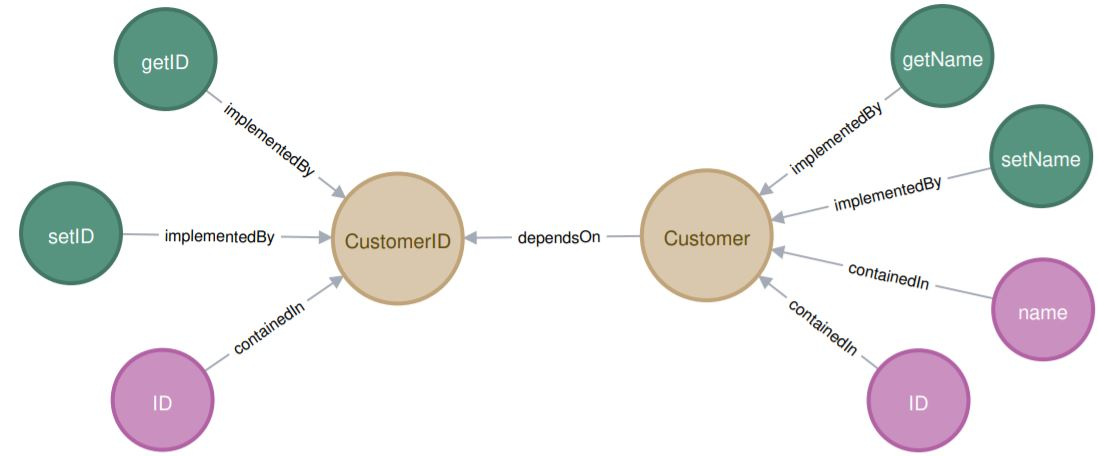
\includegraphics[scale=0.6]{Tesi/Sezione3-RiconoscimentoSmell/immagini/overengineered.JPG}
                \caption{Esempio classi overengineered nel grafo}
                \label{fig:my_label}
            \end{figure}
           
           
           \item \textit{Procedural class} classi concrete o astratte senza attributi e con solamente una oppure due funzioni definite al loro interno. Non sono state considerate nella ricerca tutte quelle classi che presentano dei supertipi, per due motivi principali. In primo luogo, se la classe avesse dei supertipi potrebbe ereditare metodi e attributi che potrebbero far sì che non rispetti più i vincoli appena definiti. Inoltre le classi procedurali sono spesso introdotte da persone non esperte nella programmazione orientata agli oggetti e prive di significato nel design, cosa che potrebbe non verificarsi se è presente una gerarchia.
            
           % Queste strategie si traducono in termini di grafo con tutti 
            Per quanto riguarda il grafo, bisogna ricercare i nodi con \textit{componentType} di valore \textit{class} oppure \textit{abstract\_class} che presentano in ingresso uno oppure due archi di tipo \textit{implementedBy} e nessun arco di tipo \textit{containedIn} in ingresso oppure \textit{isChildOf} in uscita.
        \end{itemize}
        
    %Algoritmo
    \subsubsection{Algoritmo}
        \paragraph{Input} un sottografo del grafo principale, contenente i nodi \textit{unit} e le \textit{function} e \textit{attribute} che esse definiscono. Gli archi considerati sono di tipo \textit{dependsOn}, \textit{implementedBy} e \textit{definedIn}. 
        
        \paragraph{Output} la lista delle classi affette da questo \textit{smell} e la relativa causa che ha portato alla loro identificazione. 
        
        \paragraph{Algoritmo}
            \begin{algorithmic}
    \Function{unnecessary-abstraction-detection}{G}
        \State{Prendo la lista di tutti i vertici di tipo unit}
        \For{Ogni vertice nella lista}
            %Procedural
            \If{\Call{is-procedural-class}{vertice}}
                \State{Aggiungo il vertice alla lista degli smell}
            \EndIf
            %Costant
            \If{\Call{is-constant-placeholder}{vertice}}
                \State{Aggiungo il vertice alla lista degli smell}
            \EndIf
            %Over
            \If{\Call{is-over-engineered}{vertice}}
                \State{Aggiungo il vertice alla lista degli smell}
            \EndIf
        \EndFor
    \EndFunction
    \\
    \Function{is-procedural-class}{vertice}
        \If{Il vertice è una classe concreta o astratta}
            \If{Il vertice non ha archi in ingresso containedIn}
                \If{Il vertice non ha archi in uscita isChildOf}
                    \If{Il vertice ha 1-2 archi in ingresso implementedBy}
                        \State{\textbf{return} la classe è una Unnecessary Abstraction}
                    \EndIf
                \EndIf
            \EndIf
        \EndIf
    \EndFunction
    \\
    \Function{is-constant-placeholder}{vertice}
        \If{Il vertice non rappresenta enumerazioni o classi di errore}
            \If{La classe non ha archi in ingresso implementedBy}
                \If{La classe ha archi in uscita isChildOf}
                    \If{Almeno un supertipo non è una constant placeholder op-\\\hspace{2.3cm}pure non è vuoto}
                        \State{\textbf{return} la classe non è una Unnecessary Abstraction}
                    \EndIf
                \EndIf

                \If{Tutti i nodi con arco containedIn verso questo vertice hanno \\\hspace{1.7cm} gli attributi constantAttribute e defaultValue true}
                    \State{\textbf{return} la classe è una Unnecessary Abstraction}
                \EndIf
            \EndIf
        \EndIf
    \EndFunction
    \\
    \Function{is-over-engineered}{vertice}
        \If{Il vertice ha un solo arco in ingresso containedIn}
            \If{Il vertice ha max 2 archi implementedBy in ingresso con nomi \\\hspace{1.1cm} delle funzioni collegate corrispondono a getNomeAttributo oppure \\\hspace{1.1cm} setNomeAttributo}
                \If{Il vertice ha solo un'arco in ingresso dependsOn da un vertice \\\hspace{1.7cm} che definisce un attributo dello stesso tipo della classe rappresen- \\\hspace{1.7cm}tata dal vertice}
                    \State{\textbf{return} la classe è una Unnecessary Abstraction}
                \EndIf
            \EndIf
        \EndIf
    \EndFunction
\end{algorithmic}

    